\section{Recap del contesto}
\label{sec:context}
In un contesto in cui sono sempre in maggior numero i dispositivi dotati di capacità computazionali,
che presentano la necessità di un'organizzazione e di un coordinamento tra loro,
è necessario trovare una soluzione uniforme che permetta di programmare il comportamento e la coordinazione dei dispositivi.

Questi dispositivi possono essere di natura eterogenea, ovvero possono avere architetture e sistemi operativi diversi,
e possono essere distribuiti in un'area geografica più o meno estesa.
%
La diversa natura di questi dispositivi può portare a problemi di interoperabilità e di comunicazione tra di essi.
%
Possono trovare applicazioni in vari contesti diversi, come ad esempio \emph{smart cities}, \emph{swarm robotics} e \emph{crowd management},
includendo dispositivi di tipo wearable come smartwatch e smartphone.

La gestione del singolo dispositivo in questi contesti non è banale, possono ad esempio essere presenti 200 o più dispositivi
    connessi tra loro all'interno di una rete.
%
Gestirli tutti individualmente porterebbe a problemi di scalabilità, manutenibilità ed etereogeneità.

Tra le varie soluzioni proposte troviamo l'uso del Cloud Computing o dell'Edge e Fog Computing,
    ma entrambe presentano dei problemi di scalabilità e di latenza o non sfruttano appieno le oppurtinità dell'infrastruttura.

Per questi motivi si vuole passare dall'approccio classico con device centrico, ovvero dove il programma è scritto per il singolo dispositivo,
    ad un approccio collettivo basato sulla programmazione macroscopica del comportamento dei dispositivi,
    usando tecniche di \emph{\ac{AC}}.

\ac{AC} è un paradigma di programmazione che permette di definire un unico comportamento di un insieme di dispositivi,
    definendo l'interazione fra loro.
%
È fondato sull'astrazione del \ac{FC} che consente di esprimere il comportamento auto-organizzante di reti
    di dispositivi come funzioni riutilizzabili che operano sui campi, dette ``costrutti'' o ``blocchi''.

Per fare ciò, viene sviluppato un \ac{dsl}, denominato \ck{}, basato sui concetti di \ac{AC} e \ac{FC} ed implementato in Kotlin Mulitplatform,
    che permette di scrivere codice in Kotlin e di compilarlo per diverse piattaforme, come JVM, JS, Native, iOS e Android.

\section{Lavoro svolto}\label{sec:lavoro-svolto}

Per prima cosa è servito capire quali fossero effettivamente i costrutti necessari da inserire all'interno del DSL di \ck{}.




\label{sec:contribution}
\begin{figure}
    \centering
    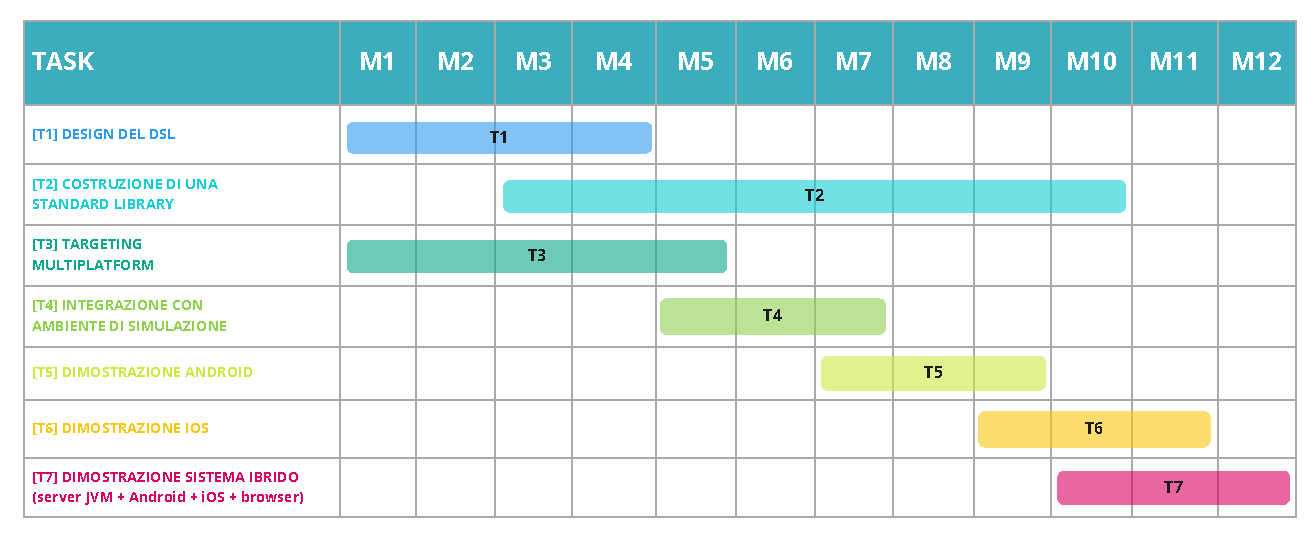
\includegraphics[width=\textwidth]{images/collektive_timeline}
    \caption{Timeline del progetto proposta.}
    \label{fig:timeline}
\end{figure}

\section{Obiettivi raggiunti}\label{sec:obiettivi-raggiunti}

\section{Prossimi obiettivi}\label{sec:prossimi-obiettivi}

